% Preprocessing implemented by #3; methodology write-up by #24.

\subsection{Preprocessing and augmentation}
\label{sec:data-preparation}

\paragraph{Standardisation.}
Each RGB channel is standardised,
\begin{equation}
  x' = \frac{x - \mu_c}{\sigma_c},
  \label{eq:standardisation}
\end{equation}
giving zero-mean, unit-variance feature scaling. Pixels are first scaled to
$[0,1]$; $\mu_c$ and $\sigma_c$ are the
per-channel mean and population standard deviation. Without this step the
three channels enter the first convolution with different offsets and spreads,
so the gradient scale differs per channel and a single learning rate suits none
of them well. The same pipeline, with the same EuroSAT statistics, feeds the
pretrained models in Task~5. Those networks were trained on standardised
inputs, but with the channel statistics of ImageNet~\cite{deng2009imagenet};
we use EuroSAT's own instead,
so that every model in the comparison sees identically preprocessed images and
the standardisation reflects the satellite data actually being classified.

\paragraph{Statistics from the training set only.}
Estimating preprocessing statistics before splitting would leak information:
if $\mu_c$ and $\sigma_c$ were computed over all
27,000 images, the preprocessing applied to the test set would already reflect
the test images, and the test score would no longer be a fair estimate of
performance on unseen data. We therefore fix the split first and estimate
$\mu_c$ and $\sigma_c$ from the training set alone (Table~\ref{tab:dataset-split}) --- before any
augmentation, at native resolution --- then apply those same values unchanged to
the validation and test sets, as an unseen deployment image would be treated.
The statistics are computed once and cached, so every experiment normalises
identically.

\paragraph{Augmentation.}
Augmentation artificially expands the size and diversity of a dataset through
transformations such as rotation and flipping. During training only, each image independently receives a horizontal
flip and a vertical flip, each with probability 0.5, and a rotation by a
uniformly chosen multiple of $90^\circ$. Together these produce all eight
orientations of the square image, freshly sampled every epoch
(Figure~\ref{fig:data-augmentation-grid}).

These transformations are \emph{label-preserving} for EuroSAT specifically. The
images are taken from directly overhead, so ``up'' in the image has no physical
meaning: a river, a highway or a field is the same land-cover class whichever
way it is rotated or mirrored. The same would not hold for ground-level
photographs, where a vertically flipped scene is not a realistic image. The
$90^\circ$ multiples are also exact pixel permutations of a square grid, so no
interpolation blurs the image and no corner is filled with padding.

Other common augmentations were deliberately not used. Random crops and
rescaling would change the apparent size of objects, but Sentinel-2 imagery has
a fixed ground resolution, so object size is real evidence --- a residential
block and an industrial site differ partly in scale --- and at $64\times64$ a
crop also discards much of a small image. Colour jitter was rejected because
colour carries the class: water, vegetation and bare soil differ chiefly in
their spectral response, so altering hue could turn one class's appearance into
another's.

\paragraph{Evaluation preprocessing and class balance.}
Validation and test images are only converted to tensors and standardised with
the training statistics, so every evaluation is deterministic. The classes are
mildly imbalanced (2,000 to 3,000 images; Table~\ref{tab:dataset-split}).
Under-sampling and synthetic minority samples are possible remedies, but at a
ratio of 1.5:1 neither was needed: stratification
keeps the imbalance identical across the three sets, and the evaluation reports
macro-averaged precision and recall alongside accuracy, so the smaller classes
are not hidden by the larger ones.

\begin{figure}[htbp]
    \centering
    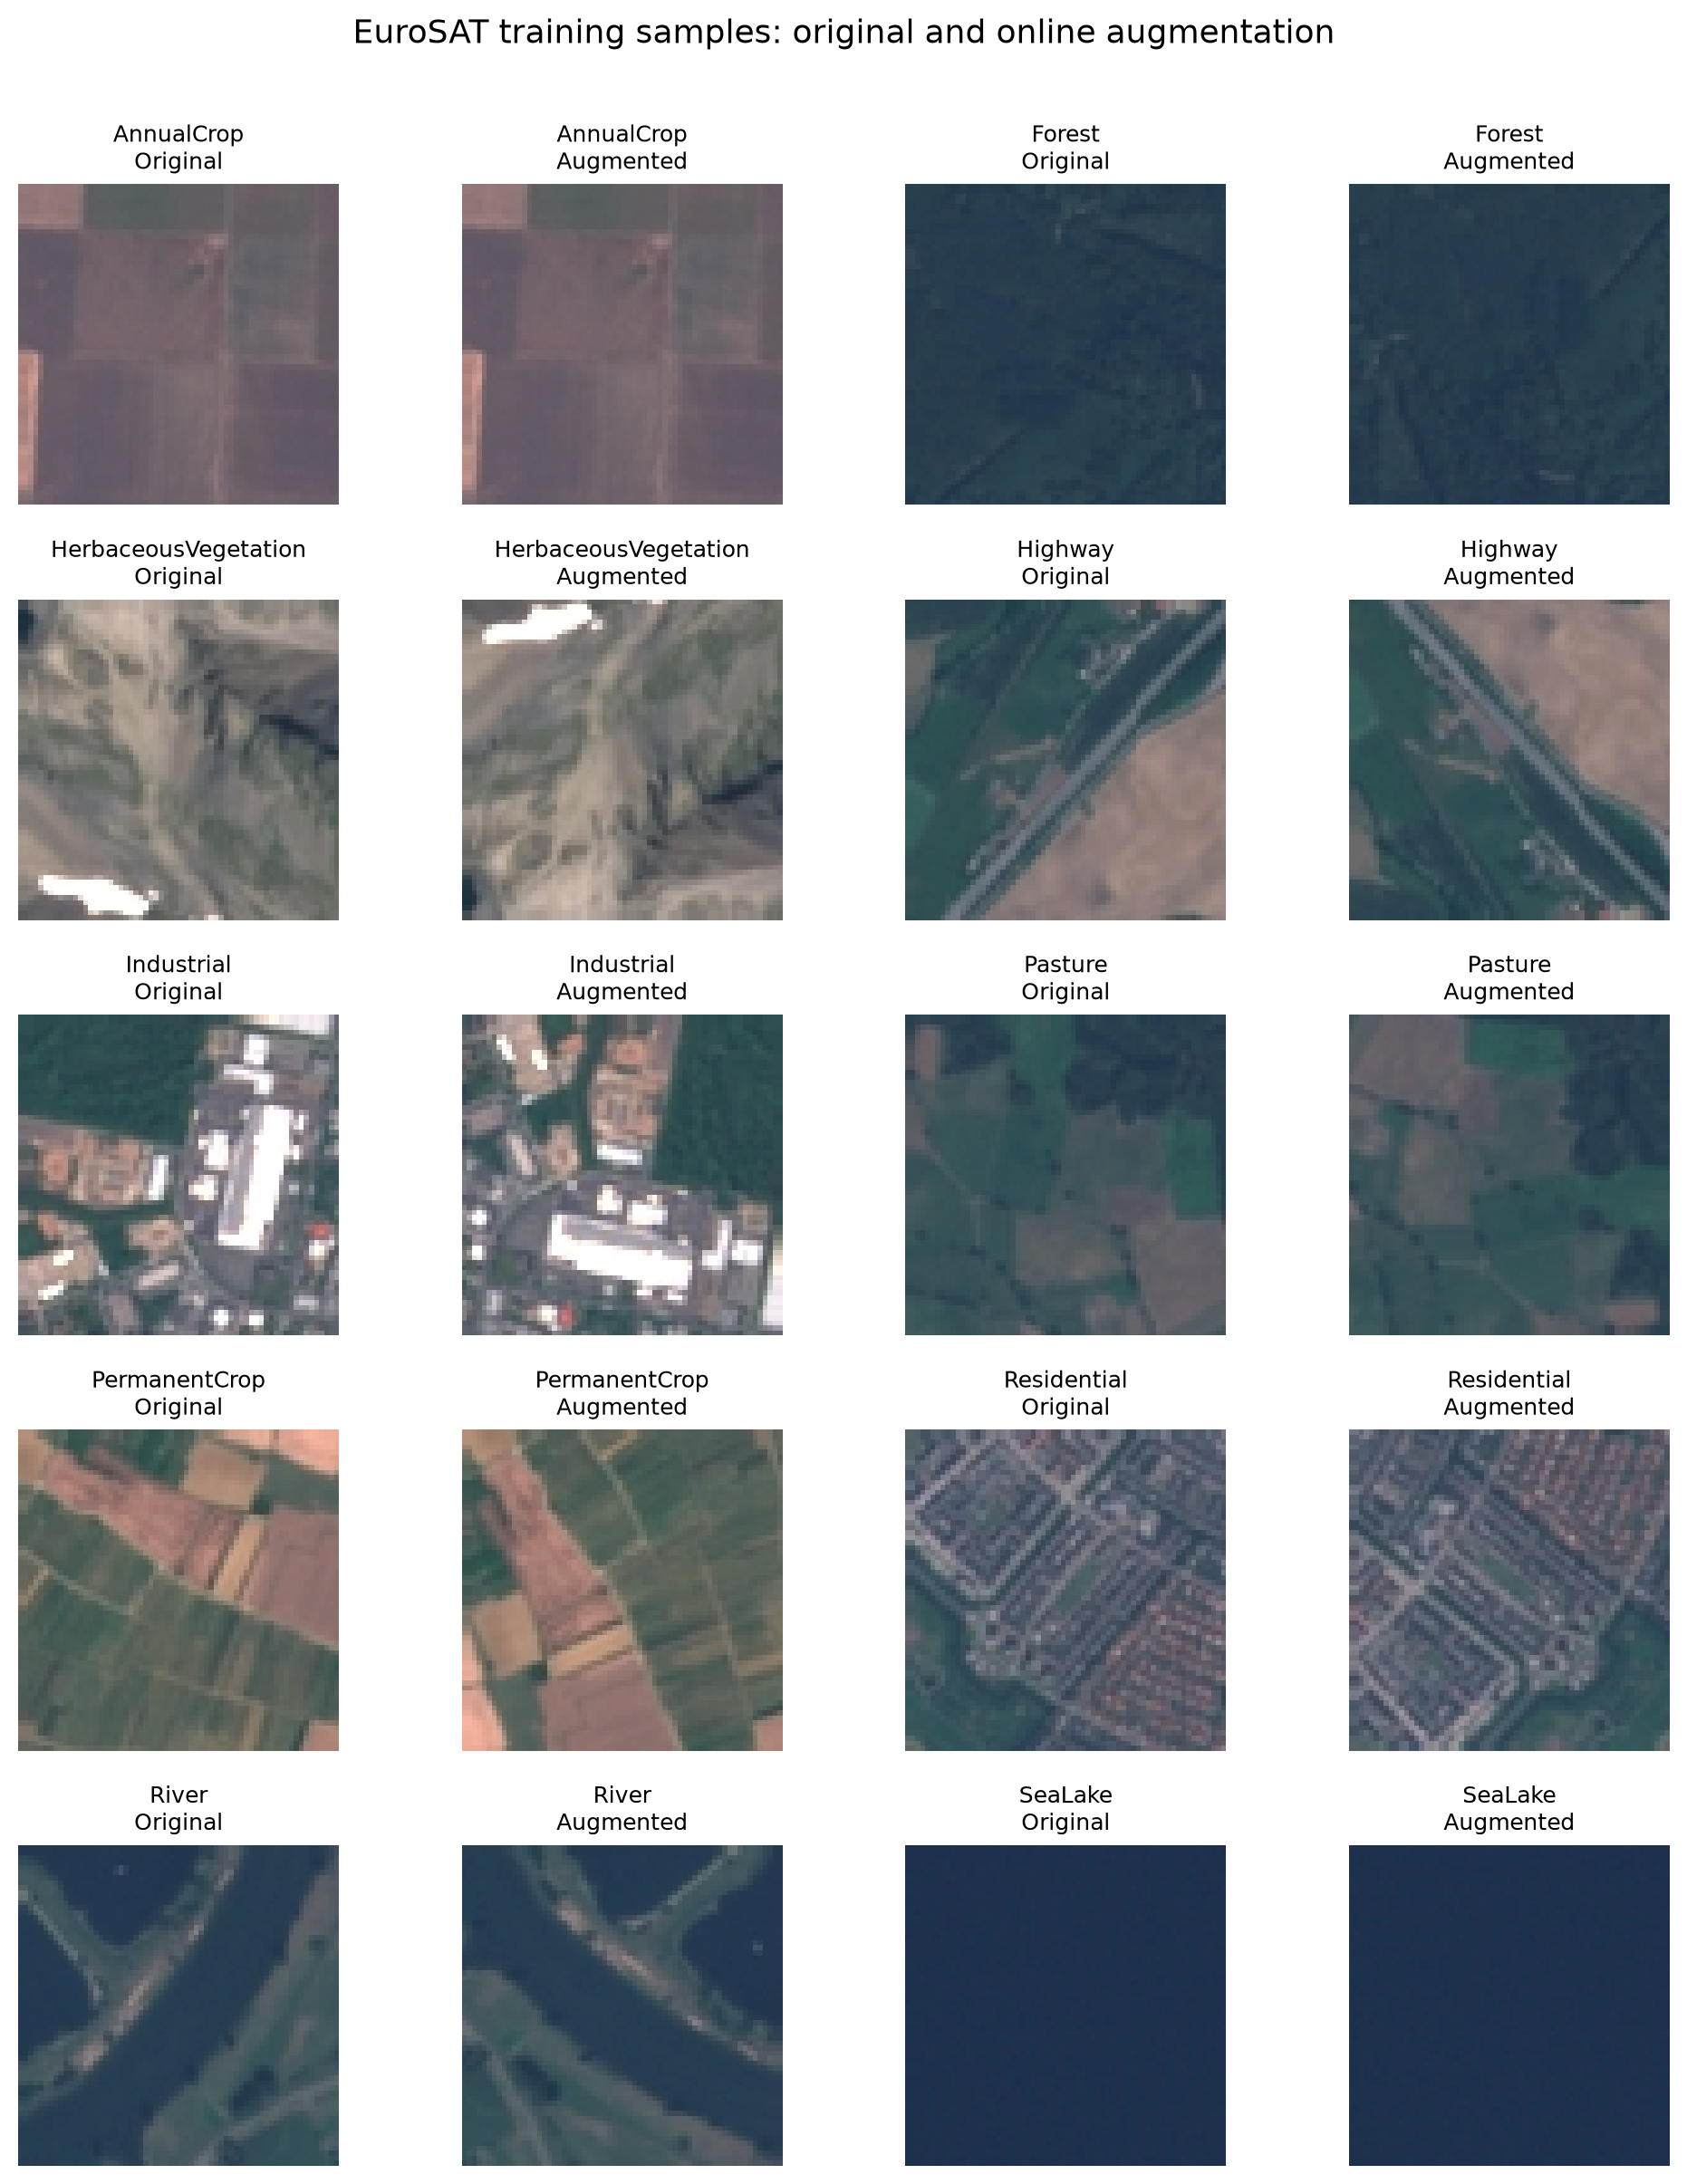
\includegraphics[width=\textwidth]{figures/data_augmentation_grid.png}
    \caption{One training image from each EuroSAT class before and after the
    configured online augmentation. EuroSAT images are natively
    $64\times64$ pixels, so these are shown at their original resolution.}
    \label{fig:data-augmentation-grid}
\end{figure}
